\section{Camada de Apresentação}

A camada de apresentação é o espaço onde ocorrem interações entre o utilizador e o serviço disponibilizado. É responsável por receber e apresentar dados ao utilizador. Tem ainda como função traduzir e enviar informação para processamento na camada lógica.

Neste sentido, foram surgindo ao longo dos anos várias \textit{frameworks} com o objetivo principal de acelarar e otimizar o desenvolvimento destes procedimentos, permitindo assim produzir uma interface de utilizador mais eficiente e agradável \textit{(user friendly)} de maneira a produzir o resultado pretendido.

Assim ao longo desta secção iremos abordar e comparar algumas das \textit{frameworks} mais utilizadas, tentando perceber no final qual delas se destaca mais entre elas. Para nos ajudar nesta análise vamos utilizar os seguintes recursos na comparação das \textit{frameworks}:

\begin{itemize}
  \item Prototipagem rápida da aplicação
  \item Complexidade
  \item Facilidade de utilização
  \item Documentação e Comunidade
  \item Ecossistema
  \item Escalabilidade
  \item Manutenção e Atualizações
  \item User Experience
\end{itemize}

\subsection{Spring MVC} % (fold)

Dos vários artigos e publicações que fomos consultando conseguímos perceber que esta \textit{framework} é das mais utilizadas na camada de apresentação.

É uma \textit{framework} concebida em torno de um \textit{DispatcherServlet} que distribui os pedidos para \textit{handlers} onde se faz o tratamento de ações. Na próxima imagem é demonstrada esta arquitetura.

\begin{figure}[ht!]
\centering
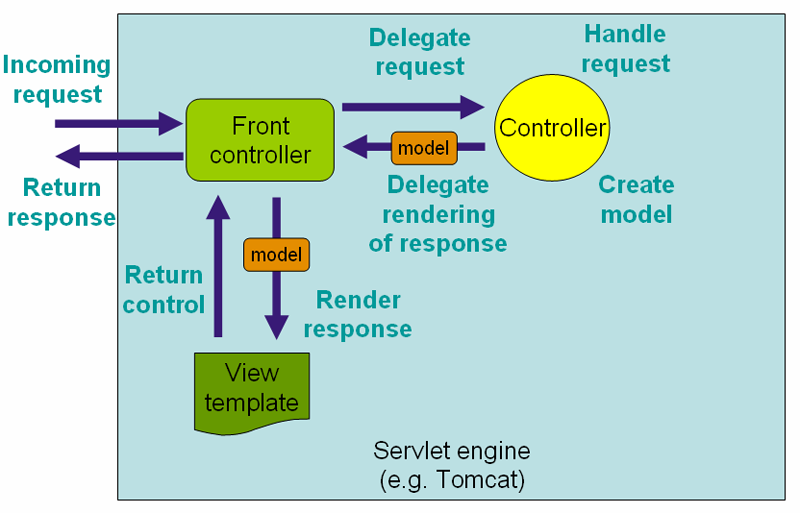
\includegraphics[width=70mm]{img/mvc.png}
\caption{Arquitetura da Framework Spring MVC}
\end{figure}

Relativamente aos aspectos, que anteriormente mencionamos, que servem de base para a avaliação da \textit{framework}, concluí-se o seguinte:

\begin{description}

\item[Prototipagem rápida da aplicação] Se estamos a procura de uma \textit{framework} que ajude a criar uma aplicação rapidamente, o Spring MVC não é o ideal. Esta \textit{framework} é enorme o que dificulta, inicialmente, a percepção da mesma.

\item[Complexidade] Spring MVC tem uma base sólida, construída ao longo dos anos, que aumenta o âmbito da sua aplicação e consequentemnete a sua complexidade.

A arquitetura da mesma é relativamente simples, mas há ainda muitas camadas e abstrações que dificultam o \textit{debug} se algum problema acontecer.

\item[Facilidade de utilização] Spring MVC não é muito fácil de utilizar, devido à grandeza e complexidade da mesma. Assim para ser utilizador desta \textit{framework} é necessário já ter alguns conhecimentos da arquitetura.

\item[Documentação e Comunidade] Como existem milhares de \textit{developers} a trabalhar com esta \textit{framework} existe muita documentação. Até o próprio site contém inúmeros tutoriais, o que é útil para iniciantes, e mesmo utilizadores avançados.

A comunidade também é muito forte, tanto a nível de suporte a dúvidas de utilizadores, como a correções de funcionalidades da \textit{framework}.

\item[Ecossistema] O ecossistema do Spring MVC é bem desenvolvida. Beneficia de ferramentas como o Spring Roo e o Spring Tool Suite IDE.

\item[Escalabilidade] Spring MVC é utilizado em aplicações de grande escala em todo o mundo. Contém os componentes necessários para o processamento em paralelo e construção de aplicações \textit{multi-thread}.

Pode ser dividida em diferentes módulos e ser configurado, mais tarde, em diferentes hosts.

\item[Manutenção e Atualizações] A manutenção de código é complicada se não forem conhecidos os pormenores da \textit{framework}.

\item[User Experience] Tem um rico conjunto de recursos para desenvolver e manter o código no servidor, mas apesar da sua extensibilidade não fornece qualquer construção de interface.

Os módulos são fáceis de gerir e criar.\\

\end{description}

Assim verifica-se que a \textit{framework} apresenta excelentes recursos de escalabilidade, ecossistema, documentação e ainda um forte apoio da comunidade. Para aplicações de baixa complexidade ou prototipagem rápida a escolha desta \textit{framework} não é a mais indicada.

%-----
\subsection{Grails}

É uma \textit{framework} para a construção de aplicações web através da linguagem dinâmica \textit{Groovy} para a plataforma Java. Grails é uma \textit{framework open-source} e pretender dar alta produtividade graças à utilização do paradigma de mais convenção e menos detalhes de configuração.

Utiliza as tecnologias que são consideradas as mais maduras do mundo de Java, como as \textit{frameworks Hibernate} e \textit{Spring}, através um interface simples e consistente.

\begin{figure}[ht!]
\centering
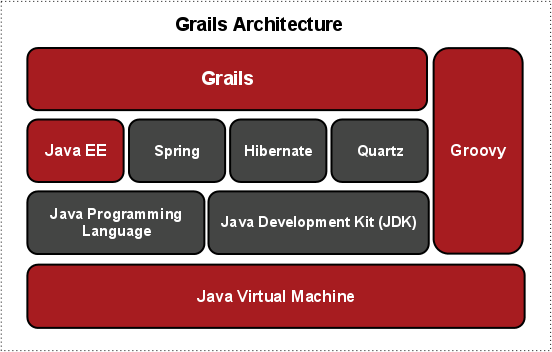
\includegraphics[width=70mm]{img/grails.png}
\caption{Arquitetura da Framework Grails}
\end{figure}

\begin{description}
\item[Prototipagem rápida da aplicação] Grails oferece uma prototipagem simples, facilitando a instalação. Possui mecanismos para geração de código automática, diminuindo o tempo de desenvolvimento.

É muito interessante utilizar esta \textit{framework} para projetos de pequena-média dimensão.

\item[Complexidade] Grails está rodeado por \textit{frameworks} de outras tecnologias como o Spring MVC e o Hibernate. Tem a mesma complexidade que estas \textit{frameworks}, acrescentado ainda uma outra camada de abstração.

\item[Facilidade de utilização] A \textit{framework} foi projetada para ser de desenvolvimento rápido e direta facilidade de utilização. Permite o uso de \textit{plugins}, através de um comando na consola todas as depedências e configurações são geradas.

\item[Documentação e Comunidade] Tem uma comunidade enorme e dedicada. Possui muita e variada documentação, inclusive, \textit{screencasts}.

\item[Ecossistema] Grails é uma \textit{framework full-stack}, onde muitas das peças fornecidas podem ser substituídas. Existe uma grande variadade de \textit{plugins} disponiveís na sua biblioteca.

\item[Escalabilidade] A \textit{framework} é uma abstração sobre Spring e Hibernate, ambos escaláveis, e sem influência no rendimento.

\item[Manutenção e Atualizações] A manutenção é fácil por não haver muita configuração e leva a que as estruturas dos projetos sejam muito semelhantes.

\item[User Experience] Os \textit{plugins} fornecidos tem fácil intregração com JavaScript e possui muitos componentes de interface.
\end{description}

Podemos concluir que esta \textit{framework} apresenta características impressionantes, que facilitam a prototipagem rápida e o desenvolvimento ágil das aplicações. Como referido anteriormente Grails é ótimo para projetos de média-baixa escala.

%-----
\subsection{GWT - Google Web Toolkit}

É um \textit{toolkit open-source} que permite aos \textit{developers} criar aplicações com tecnologia AJAX em linguagem de Programação Java.

\begin{description}
\item[Prototipagem rápida da aplicação] Possui uma quantidade enorme de \textit{widgets} para uso rápido e permite com o uso de JavaScript fazer uso de qualquer coisa.

O GWT Desgin Mode, permite através de drag-and-drop fazer uma interface fácil com geração automática de código.

\item[Complexidade] É bastante complexo. Devendo-se à enorme quantidade de código que pode ser gerada automaticamente.

\item[Facilidade de utilização] GWT possui uma estrutura bastante simples para programadores e designers. O código é fácil de interpretar e escrever.

\item[Documentação e Comunidade] Tem uma surpreendente extensa documentação oficial. O site do projeto possuí tutoriais e documentação detalhada, desde a parte mais simples à parte mais complexa.

A Google estabeleceu um conjunto de grupos de discussão que permite aos utilizadores obter suporte em questões técnicas.

\item[Ecossistema] GWT permite construir aplicações rapidamente mantendo o JavaScript do front-end com elevada perfomance em Java. O GWT SDK permite que se escreva as aplicações AJAX em java e depois compila-se o código em JavaScript.

\item[Escalabilidade] GWT foi criado para escalabilidade. O compilador Java converte JavaScript com a máxima eficiência e escalabilidade.

\item[Manutenção e Atualizações] Muito fácil de manter atualizada, mas o código gerado automaticamente pode ser díficil de interpretar.

\item[User Experience] GWT é muito versátil quando se trata de personalizar a aparência das aplicações web. É uma \textit{framework} baseada em componentes, onde a qualquer momento se pode modificar o layout sem haver uma ruptura no sistema.
\end{description}


É possível concluir que GWT é uma boa \textit{framework}, mas como se vai poder analisar mais há frente, dentro desta categoria já é possível encontrar \textit{frameworks} melhores.

%%----
\subsection{Play!}

Play! é uma \textit{framework} que torna a construção de uma aplicação web mais facilitada em Java ou Scala. É uma arquitetura muito leve e \textit{web-friendly} consumindo os recursos mínimos para aplicações altamente escaláveis.

Passando à análise das características da \textit{framework}, verifica-se:

\begin{description}
\item[Prototipagem rápida da aplicação] Play! é muito simples. Um dos objetivos de Play! é ter a mesma facilidade de criação de aplicações web que tem as aplicações em Ruby On Rails.

\item[Complexidade] Tem uma estrutura muito complexa pois existe uma vários mecanismos e módulos que podem ser movidos. É necessário ter algumas noções de Scala, caso contrário, a complexidade aumenta.

\item[Facilidade de utilização] É muito simples de começar, no entanto, fica mais complexo para os programadores mais avançados.

\item[Documentação e Comunidade] Tem uma comunidade de tamanho razoável com excelente documentação interna e externa. Existe ainda vários tutoriais a explicar as características de \textit{scaffolding}.

\item[Ecossistema] Play! oferece tudo o que é necessário para desenvolver, executar e testar as aplicações. A desvantagem real é a dependência de Scala.

\item[Escalabilidade] A \textit{framework} é incrivelmente escalável quando combinada com \textit{Acca} permitindo alta taxa de transferência.

\item[Manutenção e Atualizações] O código produzido pela \textit{framework} é legível e bem estruturado. Permite que novos utilizadores começem a trabalhar na aplicação sem perder demasiado tempo a perceber o funcionamento da mesma.

\item[User Experience] Possuí alguns temas básicos, no entanto não há um apoio generalizado para bibliotecas de componentes.
\end{description}

%----
\subsection{JSF - JavaServer Faces}

JavaServer Faces (JSF) é uma framework MVC baseada em Java para a construção de interfaces baseadas em componentes para aplicações web. Tem um modelo de programação direcionado a eventos, abstraindo os detalhes da manipulação dos eventos e organização dos componentes.

\begin{figure}[ht!]
\centering
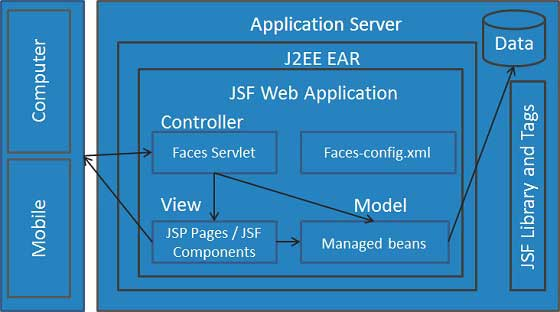
\includegraphics[width=70mm]{img/jsf.jpg}
\caption{Arquitetura da Framework JSF}
\end{figure}

Obteve-se as próximas conclusões, relativas às características definidas inicialmente.

\begin{description}
\item[Prototipagem rápida da aplicação] JSF não é a melhor para a elaboração rápida de protótipos pois exige tanto de configuração como uma aplicação completa.

Os maiores ganhos na produtividade com JSF são os assistentes disponíveis na maioria dos IDEs que geram a maior parte do código.

\item[Complexidade] É muito complexa, derivado à complexidade da especificação JAVA EE.

\item[Facilidade de utilização] JSF tenta proporcionar uma estrutura fácil de utilização para a criar componentes web reutilizáveis nas aplicações Java.

As ferramentas da \textit{framework} tornam mais fácil a utilização e não possui depedências externas enquanto estivermos dentro do ecossistema Java EE, que JSF aproveita bem.

\item[Documentação e Comunidade] JSF é totalmente suportado pela Oracle. Ao contrário de outras \textit{frameworks} JSF tem funcionários para escrever documentação e criar amostras e exemplos.

A única desvantagem da documentação da Oracle é a dependência do seu IDE e Application Server.

\item[Ecossistema] Porque é parte da especificação de Java EE, JSF recebe todos os benefícios e ferramentas Java EE. Incluíndo suporte para IDEs com muitas funcionalidades.

\item[Escalabilidade] As aplicações JSF podem ser realizadas, mas os ganhos de desempenho vêm do cluster de servidores de aplicações Java EE. O próprio JSF não fornece suporte explícito para chamdas assíncronas.

\item[Manutenção e Atualizações] Um dos objetivos de JSF é ajudar os programadores a produzir um código melhor.

\item[User Experience] As bibliotecas de construção de componentes está cheia de recursos e há um extenso catálogo \textit{3rd-party} disponíveis.
\end{description}

%----
\subsection{Outras frameworks}

Derivado à grande quantidade de \textit{frameworks} existentes para a camada de apresentação não foi possível apresentar todas as características e explicações das mesmas.

Merecem ainda algum destaque as seguintes \textit{frameworks}:

\begin{description}

\item[Struts] É uma \textit{framework} baseada em ações que segue o padrão Model 2, que é uma variação complexa do padrão MVC.

\item[Wicket] Desenvolvida pela Apache FOundation, é semelhante ao JavaServer Faces (JSF). Caracteriza-se por centralizar em POJO (Plain Old Java Objects) e evitar o excesso de ficheiros de configuração em XML.

\item[Vaadin] É uma \textit{framework} desenvolvida a partir da \textit{framework} GWT - Google Web Toolkit. Esta opera no lado do servidor, embora também funcione no lado do cliente, recorrendo a tecnologia AJAX.

\end{description}

%----
\subsection{Decisão Final}

Depois de feita a comparação entre as várias características existentes numa \textit{framework} foi feita a escolha de uma, que neste caso completa mais os tópicos analisados.

Para nos ajudar nesta escolha recorremos ao artigo da RebelLabs que analisou cuidadosamente as características de várias \textit{frameworks} e atribuíu pontuações às mesmas.

\newpage

\begin{figure}
\centering
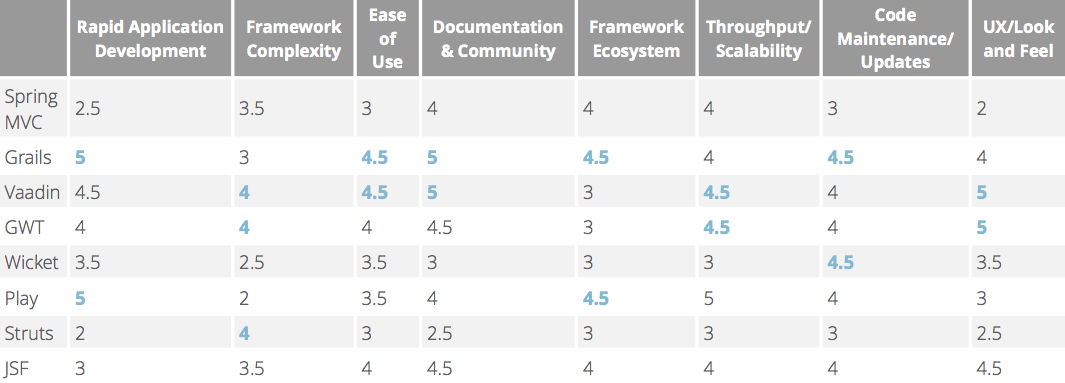
\includegraphics[width=130mm]{img/frams.png}
\caption{Análise das frameworks}
\end{figure}

Com a seguintes pontuações totais ordenadas:

\begin{figure}[ht!]
\centering
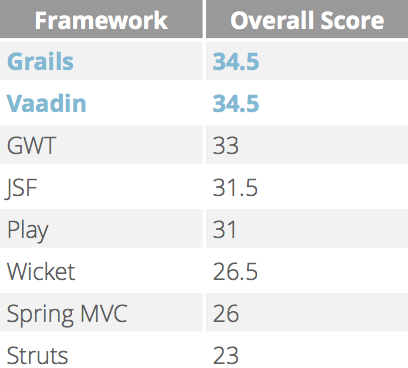
\includegraphics[width=60mm]{img/tot.png}
\caption{Pontuações obtidas por Framework}
\end{figure}


Estas tabelas refletem que as \textit{frameworks Grails e Vaadin}, apresentam-se como as mais completas nos tópicos analisados anteriormente.

A \textit{framework Grails}, através da análise das tabelas anteriores mostrou que para as 8 categorias analisas ela é bastante completa em 5. Particularmente em desenvolvimento rápido de aplicações, documentação e comunidade, com as melhores notas. O tópico que ficou mais abaixo dos valores foi nas comparações de complexidade, este valor reflete as depedências com Spring e Groovy, mais a adição de camadas de abstração.

A \textit{framework Vaadin}, como verificado nas tabelas anteriores esteve muito bem em 3 categorias. Apesar de não termos efetuado uma comparação exaustiva da mesma, serve para demonstrar que é uma boa \textit{framework} de desenvolvimento. Esta saiu mais destacada na análise de User Experience e também na documentação e comunidade.

Estas duas \textit{frameworks} são uma excelente opção para projetos de pequena-média dimensão, no entanto também se enquadram em grandes dimensões devido à sua escalabilidade e desempenho.

Concluí-mos então que as duas frameworks faladas em cima são as melhores para a análise efetuada.
